\section{Расчёт прохождения нейтрино через Землю}
\label{sec:zfactor}
В работе используется модель PREM для описания плотности вещества Земли (см. приложение~\ref{sec:prem}). Расчёт глубины 
\[
X=\int\limits_\text{траектория}\rho(\ell) d\ell
\]
осуществляется численным интегрированием плотности вдоль траектории нейтрино.

\subsection{$\mathcal{Z}$-факторный метод}

$\mathcal{Z}$-фактор представляет собой поправку к затуханию потока нейтрино, учитывающую регенерацию за счёт нейтрального тока. Метод предложен и подробно описан в работе~\cite{naumov1999} и базируется на решении следующего уравнения переноса нейтрино:
\begin{equation}
\frac{\partial F_{\nu}(X,E_\nu)}{\partial X} = \frac{1}{\lambda_{\nu}(E_\nu)}\left[ \int\limits_0^1\frac{dy}{1-y}\Phi_{\nu}(y,E_\nu) F_{\nu}(X,E_y) - F_{\nu}(X,E_\nu) \right],
\end{equation}
где $F_{\nu}(X,E_\nu)$ — поток нейтрино после прохождения глубины $X$, $E_y = E_\nu/(1-y)$, 
\[
\lambda^{-1}_{\nu}(E_\nu) = \sum\limits_{T\in \{n,p,e\}}n_T\sigma_{\nu T}^{tot}(E)
\] 
- пропорционально полному сечению взаимодействия нейтрино с веществом, а $\Phi_{\nu}(y,E)$ — распределение по передаче энергии, определяемое следующей формулой:
\begin{equation}
    \Phi_{\nu}(y,E_\nu) = \frac{\sum\limits_{T\in \{n,p,e\}}n_T\frac{d\sigma_{\nu T}}{dy}(y,E_y)}{\sum\limits_{T\in \{n,p,e\}}n_T\sigma_{\nu T}(E_\nu)}.
\end{equation}
В этих формулах $n_T$ число мишеней на грамм вещества.

Искомое решение имеет вид:
\begin{equation}
F_{\nu}(X,E_\nu) = F^{0}_{\nu}(E_\nu)\exp\left(-\frac{x}{\Lambda_{\nu}(X,E_\nu)}\right),
\end{equation}
где 
\begin{equation}
\Lambda_{\nu}(X,E_\nu) = \frac{\lambda_{\nu}(E_\nu)}{1 - \mathcal{Z}_{\nu}(X,E_\nu)}.
\end{equation}

Решение уравнения для $\mathcal{Z}_{\nu}(X,E_\nu)$ реализуется итерационно, начиная с $\mathcal{Z}^{(0)}$ и строя следующие приближения по схеме:
\begin{equation}
\mathcal{Z}^{(n+1)}_{\nu}(X,E_\nu) = \int\limits_0^X dX' \int\limits_0^1 dy\,\eta_{\nu}(y,E_\nu)\Phi_{\nu}(y,E_\nu)\exp\left[ -X'D^{(n)}_{\nu}(X',E_\nu,E_y) \right],
\end{equation}
где $\eta_{\nu}(y,E_\nu)$ — весовой фактор, определяемый формой начального спектра. Точное выражение для $\eta_{\nu}(y,E_\nu)$ имеет следующий вид: 
\begin{equation}
    \eta_{\nu}(y,E_\nu) = \frac{F^0_{\nu}(E_y)}{(1-y)F^0_{\nu}(E_\nu)}.
\end{equation}
Выражение для фактора $D^{(n)}_{\nu}(x, E_\nu, E_y)$ имеет следующий вид:
\begin{equation}
    D^{(n)}_{\nu}(X, E_\nu, E_y) = \frac{1-\mathcal{Z}_{\nu}^{(n)}(X, E_y)}{\lambda(E_y)} - \frac{1-\mathcal{Z}_{\nu}^{(n)}(X, E_\nu)}{\lambda(E_\nu)}.
\end{equation}
Решение уравнения переноса для потока нейтрино учитывает как исчезновение нейтрино за счёт заряженного тока, так и эффект регенерации от нейтрального тока. 

\subsection{Непрозрачность Земли}
Иллюстрация решения $\mathcal{Z}$-факторным методом приведена на  рис. (\ref{EF2}). Здесь показано отношение потока нейтрино $F_\nu(X(\theta),E_\nu)$  после прохождения вещества Земли к потоку $F_\nu^0(X(\theta),E_\nu)$ на поверхности Земли. Это  отношение можно считать приближением к вероятности прохождения нейтрино.
\begin{figure}[!h]
\centering
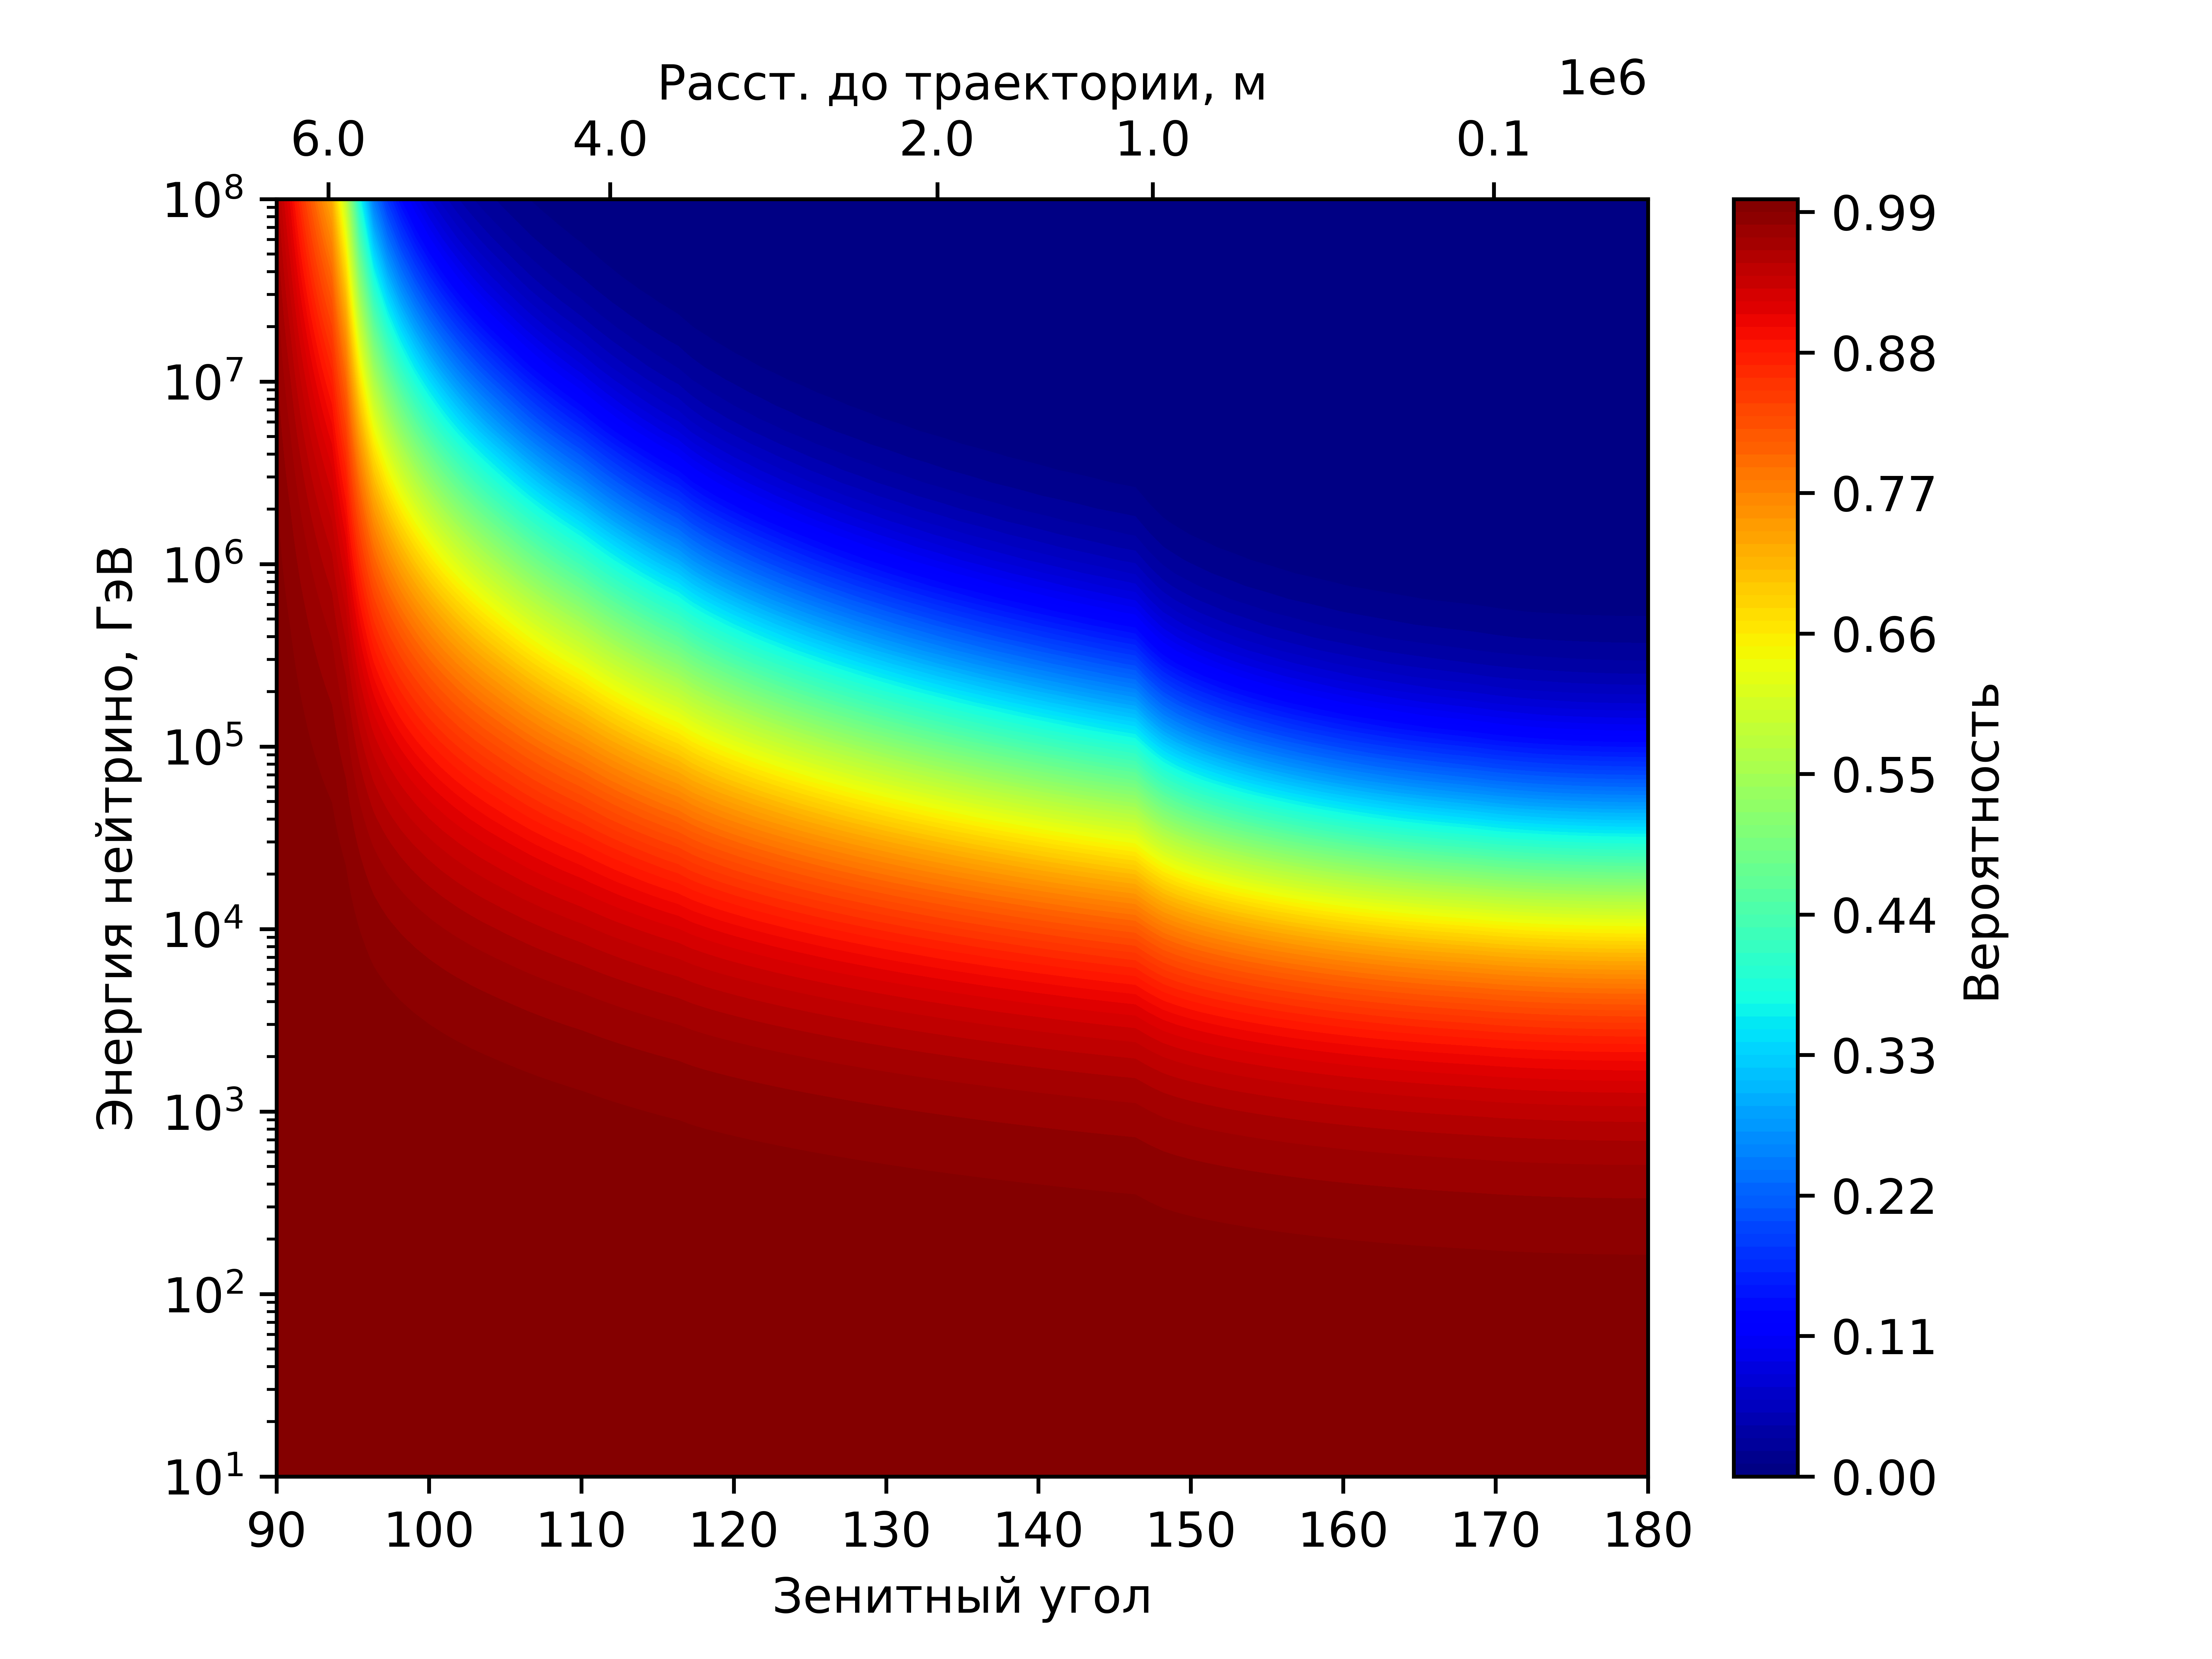
\includegraphics[width=0.8\linewidth]{images/NuProp/rzf_2dxsCT10nlo.png}
\caption{Вероятность прохождения нейтрино сквозь Землю в зависимости от энергии и зенитного угла, измеряющегося относительно детектора.}
\label{EF2}
\end{figure}
Тёмно-синия область на рис.~(\ref{EF2}) отвечает ситуации когда Земля становится практически непрозрачной для нейтрино.

Для вычисления графика~(\ref{EF2}) использовалась следующая модель спектра нейтрино:
\begin{equation}
    F_{\nu}^{0}(E) = K\left(\frac{E_0}{E}\right)^{\gamma+1} (1+E_0/E)^{-\alpha},%\phi\left(\frac{E}{E_{cut}}\right),
\end{equation}
с параметрами $\gamma = 1$ и $\alpha = 0.5$. 
% $\phi_{cut}(t)$ - некоторая функция, предназначенная для обрезания потоков при энергиях выше некоторого порога. В настоящей работе использована:
% \begin{equation}
%     \phi(t) = (1+\tan(\pi t/2))^{-1}
% \end{equation}
